% !TeX encoding = utf8
% !TeX spellcheck = fr

\chapter{Interface utilisateur}\label{cha:interface}

\begin{figure}[h]
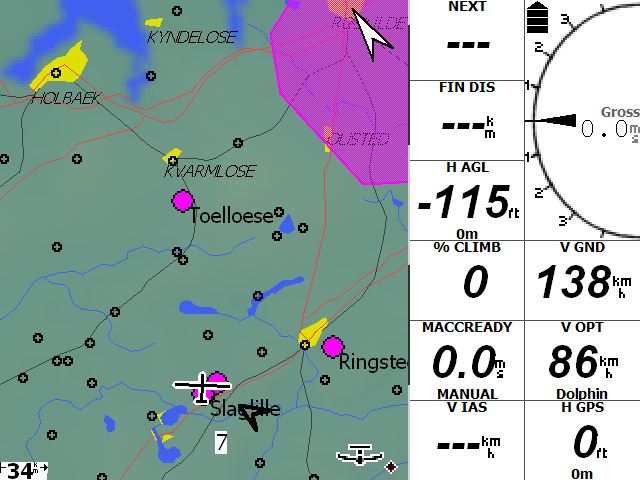
\includegraphics[angle=0,width=\linewidth,keepaspectratio='true']{figures/plain.png}
\caption{Disposition typique de l'écran principal d'\xc{}}
\end{figure}

Ce chapitre décrit les concepts de base de l'interface utilisateur d'\xc{}
et est pensé comme une vue d'ensemble. L'\emph{écran principal} contient la majorité
des informations nécessaires à un vol normal. Habituellement, l'écran principal est
constitué d'une carte mobile et d'Infoboxes. Pour différentes raisons --- qui sortent du
cadre de cette introduction --- vous pouvez, lors d'un vol choisir d'utiliser plusieurs écrans principaux
appelés \emph{pages d'écran}.

\begin{framed}
	\begin{center}
		\xc{} est entièrement développé par des bénévoles.\\
		Cette documentation aussi.\\
		Si vous y voyez des imperfections, vous pouvez facilement les faire disparaître~:\\
		\xcsoarwebsite{/develop/}
	\end{center}
\end{framed}

Les pages d'écran sont facilement accessibles par une saisie tactile du type balayage horizontal
similaire à celui utilisé pour tourner les pages d'un libre, ou par l'appui sur un bouton, selon l'appareil que vous utilisez.
Avec les pages d'écran, vous pouvez créer plusieurs écrans principaux
utiles dans différentes phases de vol. Dit autrement, vous avez
accès aux informations appropriées dans différents \emph{cas d'usage}, et ce
avec un accès simple et rapide.

Dès que la situation présente nécessite d'attirer l'attention du pilote, une
\emph{incrustation} est affichée par dessus l'écran principal. Cela survient en particulier
quand une réaction rapide est attendu de la part du pilote, telle qu'une
possible collision ou l'entrée imminente dans un espace aérien réglementé.

Bien évidemment, les boutons du menu et les écrans de menu sont aussi en incrustation,
et ils sont nombreux. En conséquence, les éléments superposés constituent d'une pile d'affichage dont
l'écran principal représente la couche de base. Des descriptions plus détaillées sont
données dans les chapitres suivants.

\section{Éléments de l'affichage}
\subsection*{Écran principal et pages d'écran}
Chacune des pages d'écran de l'ensemble des pages d'écran d'\xc{} se compose de plusieurs
parties~:
\begin{description}
\item[Zone principale] La plus grande partie de l'écran est habituellement dédiée à l'affichage
de la carte mobile GPS. Différents symboles reprenant des informations de l'ordinateur de vol sont surimposés
à cette carte. Des icônes et du texte peuvent apparaître sur le bord inférieur de l'écran
afin d'indiquer le statut des périphériques connectés, les modes de vols, etc.
Dû au processus de développement d'\xc{}, il existe un nombre croissant
d'éléments qui peuvent être sélectionnés afin de les afficher sur la zone principale, tels que des jauges,
le radar \fl, l'assistant thermique et l'horizon artificiel.
\item[InfoBoxes] Une grille de valeurs est habituellement affichée soit le long des bords supérieur et inférieur 
de l'écran (affichage en mode portrait), soit sur la droite et la gauche de
l'écran (affichage en mode paysage). Ces ``Infoboxes'' affichent des données en provenance du
GPS et d'autres capteurs, ainsi que des valeurs calculées par \xc. De plus,
des InfoBoxes peuvent aussi afficher des jauges, voire des graphes.
\item[Zone inférieure] Sur le bas de l'écran, \xc{} est capable de dessiner une coupe
verticale du relief et des espaces aériens dans la direction de votre déplacement.
\end{description}

\subsection*{Incrustations}
\begin{description}
\item[Jauges] Les jauges fournissent des affichages ressemblant à des instruments. Toutes les jauges sont optionnelles
et certaines ne fourniront des informations utiles que lorsqu'\xc{} sera
connecté à un périphérique pris en charge.
Une inscrustation sous forme de jauge peut soit être affichée en continu, soit s'afficher
lorsque différentes conditions sont remplies. Par exemple, l'assistant thermique ne s'affiche que lorsqu'\xc{} est en mode
thermique. Le radar \fl{} ne s'affiche que lorqu'une collision potentielle est détectée.
Les inscrustations permanentes sous forme de jauge sont par exemple la barre d'arrivée et
la barre du vario.
\item[Étiquettes de bouton et menus] Les boutons physiques présents sur l'appareil faisant tourner \xc{}
peuvent être utilisés pour activer les menus de l'écran et y naviguer. Ils sont
habituellement disposés de façon à ce que les éléments d'un menu puissent être sélectionnés en appuyant
sur le bouton adjacent à l'élément. Si l'appareil dispose d'un écran tactile, les éléments d'un menu
peuvent être sélectionnés en appuyant dessus. Ces boutons ont un fond gris avec du texte noir.
\item[Messages d'état] Du texte est affiché sur l'écran dans une fenêtre de message
d'état. Ce texte est utilisé pour donner des informations détaillées au pilote lorsque
certains évènements surviennent.
\item[Fenêtre de dialogue] Des fenêtres de dialogue plus grandes, contenant habituellement des graphiques et
des boutons, sont utilisées pour fournir au pilote des données détaillées concernant un point
de virage, des statistiques, des analyses, etc.
\item[Menu principal] Le menu principal est accessible en tapotant deux fois la carte ou
les InfoBoxes, ainsi qu'à travers des saisies tactiles. Si les boutons du menu ne sont pas activés après 
\gesturespec{du} une durée donnée, ils disparaissent afin de ne pas masquer
la carte.
\end{description}



\subsection*{Jauge de vario classique}
Comme dit précédemment, des jauges peuvent être affichées de différentes façons, soit dans une
InfoBoxe, soit en incrustation, voire même dans la zone principale. La jauge de vario traditionnelle est
différente. La jauge de type aiguille est affichée en permanence en choisissant une disposition
d'InfoBoxe qui inclue ce variomètre sur le coté droit des autres InfoBoxes.

\section{Interaction}
Il y a différentes façons d'interagir avec XCSoar~:
\begin{itemize}
\item toucher certains éléments de la carte
\item toucher des InfoBoxes et des boutons de menu à l'écran
\item par geste, par exemple en dessinant un trait allant de la gauche vers la droite 
de l'écran (voir Section~\ref{sec:gestures}).
\item ``déplacer'' l'affichage (en touchant l'écran, puis en glissant avant de relâcher).
\item appuyer sur des boutons d'application de l'appareil.
\item appuyer sur les touches de curseur de l'appareil.
\item appuyer sur les touches ou les interrupteurs d'un périphérique connecté à \xc.
\end{itemize}
Selon l'appareil particulier qui est utilisé avec \xc, seulement une partie de ces méthodes
d'interaction sont possibles et il pourrait y avoir différents nombres ou affectations
de boutons.

Pour la version PC de \xc, cliquer avec la souris sur un élément est équivalent à
le toucher.

\section{Le menu principal}
Le menu principal est une série de boutons dessinés sur l'écran et activés en les tapotant
ou en appuyant sur un bouton de l'appareil. Utiliser ces boutons et le menu principal est la façon
principale qu'à l'utilisateur pour interagir avec \xc.

\subsection*{Bases sur l'interface}
Le menu est organisé en quatre différents groupes de fonctions, habituellement sous
une forme de hiérarchie. La disposition particulière du menu dépend de la configuration
des bouton de l'appareil et du système d'exploitation. Cette disposition peut aussi être modifiée par
l'utilisateur.

\xc{} peut aussi recevoir des instructions de claviers externes, game pads, manettes de jeux, 
boutons situés sur le manche, etc. Un grand nombre de fonctions peuvent être assignées à ces
périphériques externes.
\sketch{figures/buttonmenu.png}

Sur la version PC, ces boutons de mode sont activés par les
touches 1, 2, 3 et 4. Les touches 6, 7, 8, 9 et 0 correspondent à la bande
horizontale de boutons.

Si l'utilisateur n'interagit pas avec l'ordinateur pendant un certain temps, le
menu disparaîtra automatiquement. Cette durée d'affichage du menu est configurable.
La touche d'échappement sur un PC peut aussi être utilisée pour fermer le menu actuel.

Les boutons du menu apparaissent en grisé si la fonction correspondante n'est pas disponible.
Par exemple, la fonction ``Liste des points de virage'' sera grisée si aucun point de virage n'a été chargé.

Plusieurs étiquettes de boutons du menu ont un texte se modifiant selon le contexte, ce qui
permet de clarifier ce qui arrivera lorsque le bouton sera
pressé.
La convention est que l'étiquette d'une bouton décrive ce qu'il
se produira quand le bouton sera pressé. Par exemple, si l'on considère le bouton
\bmenug{MC Auto}, le presser démarrera le ``MacCready Auto',
et l'étiquette du bouton sera modifiée en \bmenug{MC Manuel}. 
Dans la liste des menus décrits ci-dessous, des étiquettes génériques sont utilisées.

\subsection*{Groupes de fonction du menu}
Ce paragraphe décrit la disposition par défaut de système de menus de toutes
les plateformes. Les fonctions effectuées par chaque bouton sont expliquées plus
en détails dans les chapitres suivants. 

Pour la version PC, les touches~1, 2, 3 et 4 activent le
menu correspondant. La liste ci-dessous des éléments du menu dispose sur le coté gauche
de la plupart des boutons du menu de liens vers le paragraphe particulier. Suivez-les pour obtenir
tous les détails y référents.

\section{Vue générale des éléments des menus}

\subsection*{Menu Navigation}
\noindent\makebox[\textwidth]{%
	
\begin{tabularx}{1.44\textwidth}{c|ccccc}
\bmenus{Nav. 1/2}
 & \bmenus{Circuit}
 & \bmenut{Point virage}{précédent}
 & \bmenut{Point virage}{suivant}
 & \bmenut{Liste des}{points virage}
 & \bmenus{Dégagmts} \\
Voir~:
 & \ref{cha:tasks}
 & \ref{sec:advanc-rest-tasks}
 & \ref{sec:advanc-rest-tasks}
 & \ref{sec:waypoint-selector-dialog}
 & \ref{sec:alternates} \\ \\
\bmenus{Nav. 2/2}
 & \bmenut{Circuit}{Abandon}
 & \bmenus{Marquer}
 & \bmenus{Objectif}
 & {}
 & {} \\
Voir~:
 & \ref{sec:taskabort}
 & \ref{sec:markers}
 & \ref{sec:waypointdetails}
\end{tabularx}}

Vous ne devriez pas commencer à utiliser \xc{} sans connaître d'abord la fonctionnalité ``Dégagements'. 
Tout élément lié à un ``circuit'' dans le menu de navigation est utilisé pour planifier un vol
sur la campagne, et c'est certainement la deuxième chose à connaître.

\subsection*{Menu Affichage}
\noindent\makebox[\textwidth]{%

\begin{tabularx}{1.44\textwidth}{c|ccccc}
\bmenus{Affich. 1/2}
 & \bmenus{Zoom}
 & \bmenus{Dézoom}
 & \bmenut{Zoom}{Auto}
 & \bmenut{Info.}{Thermique/...}
 & \bmenut{Panor.}{ON} \\
Voir~:
 & \ref{sec:zooming}
 & \ref{sec:zooming}
 & \ref{sec:zooming}
 & \ref{sec:screenpages}
 & \ref{sec:panning} \\ \\
\bmenus{Affich. 2/2}
 & \bmenut{Étiquettes}{Tous/...}
 & \bmenut{Trace}{Complet/...}
 & \bmenut{Relief}{On/Off}
 & \bmenut{Topo.}{On/Off}
 & \bmenut{Espace aérien}{On/Off} \\
Voir~:
 & \ref{sec:maplabels}
 & \ref{sec:trail}
 & \ref{sec:terrain_topo}
 & \ref{sec:terrain_topo}
 & \ref{sec:terrain_topo}
\end{tabularx}}

La plupart des éléments du menu Affichage sont accessibles par saisie tactile ou par les touches spéciales
de raccourcis de votre appareil. Une fois que vous seriez familiarisé avec \xc{}, vous utilisez probablement
ces éléments du menu moins fréquemment.

\subsection*{Menu Configuration}
\noindent\makebox[\textwidth]{%

\begin{tabularx}{1.44\textwidth}{c|ccccc}
\bmenus{Config. 1/3}
 & \bmenut{MacCready}{$+$}
 & \bmenut{MacCready}{$-$}
 & \bmenut{MacCready}{Auto}
 & \bmenus{Vol}
 & \bmenus{Vent} \\
Voir~:
 & \ref{sec:stf}
 & \ref{sec:stf}
 & \ref{sec:auto-maccready}
 & \ref{sec:flight-setup}
 & \ref{sec:wind-setup} \\ \\
\bmenus{Config. 2/3} 
 & \bmenus{Système}
 & \bmenus{Planeur}
 & \bmenus{Périph.}
 & \bmenut{Gestionnaire}{de fichiers}
 & \bmenus{Rejouer} \\
Voir~:
 & \ref{cha:configuration}
 & \ref{sec:glidepolar}
 & \ref{conf:comdevices}
 & {}
 & \ref{sec:logger-replay} \\ \\
\bmenus{Config. 3/3} 
 & \bmenut{Enregistr.}{Démarrer}
 & \bmenus{Logger brut}
 & \bmenus{Airspace}
 & \bmenus{Vega}
 & \bmenus{Profils} \\
Voir~:
 & \ref{sec:logger}
 & \ref{sec:raw-logger}
 & \ref{sec:airspace-filter}
 & {}
 & {}
\end{tabularx}}

Le menu Configuration fait typiquement partie des paramétrages d'\xc{}
effectués au sol. Vous n'êtes pas sensé, une fois en vol, passer du temps à ajuster
la configuration, excepté pour ajuster manuellement les paramètres du vent ou du MacCready.
L'élément ``Vega'' donne contrôle sur le variomètre intelligent Vega. Cela
inclut un sous-menu.

\subsection*{Menu Information}
\noindent\makebox[\textwidth]{%

\begin{tabularx}{1.44\textwidth}{c|ccccc}
\bmenus{Info. 1/3}
 & \bmenut{Radar}{Flarm}
 & \bmenut{METAR}{TAF}
 & \bmenut{Qu'y a-}{t'il ici ?}
 & \bmenut{Check}{liste}
 & \bmenus{Analyses} \\
Voir~:
 & \ref{sec:flarm-traffic}
 & \ref{sec:metar-taf}
 & {}
 & \ref{sec:checklist}
 & \ref{sec:analysis-climb} \\ \\
\bmenus{Info. 2/3}
 & \bmenus{États}
 & \bmenus{Météo}
 & \bmenus{Équipe}
 & \bmenus{Liste du trafic}
 & \bmenut{Assistant}{Thermique} \\
Voir~:
 & \ref{sec:flight-status}
 & \ref{sec:weather-forecast}
 & \ref{sec:team-flying}
 & {}
 & \ref{sec:thermal-assistant} \\ \\
\bmenus{Info. 3/3}
 & \bmenus{Crédits}
 & \bmenus{Espaces aériens}
 & \bmenut{Répéter}{Message}
 & {}
 & {} \\
Voir~:
 & \ref{sec:credits}
 & 
 & 
 & 
 &
\end{tabularx}}

Le menu Information est toujours une source précieuse quand vous avez besoin de plus
que de configurer votre MacCready~; par exemple, lorsque vous avez besoin d'une aide élaborée sur votre vol
par rapport à une décision tactique de grande portée.

\subsection*{Le sous-menu Variomètre Vega dans le menu Configuration}
\noindent\makebox[\textwidth]{%

\begin{tabularx}{1.44\textwidth}{c|ccccc}
\bmenus{Vega 1}
 & \bmenut{Boutons}{Cockpit}
 & \bmenut{Options}{Audio}
 & \bmenut{Demo}{manuel}
 & \bmenut{Configuration}{Décrochage}
 & \bmenus{Accel} \\ \\
\bmenus{Vega 2}
 & \bmenut{ASI}{zéro}
 & \bmenut{Accel}{zéro}
 & \bmenus{Enregistrer}
 & \bmenut{Démo}{Transition}
 & \bmenut{Démo}{Montée}
\end{tabularx}}

Les fonctions de ce sous-menu nécessitent le variomètre Vega intelligent.
Le menu est accessible uniquement si ``Vega'' est sélectionné comme périphérique connecté.

\subsection*{Le sous-menu Panorama du menu Affichage}

\noindent\makebox[\textwidth]{%

\begin{tabularx}{1.44\textwidth}{c|ccccc}
\bmenus{Panor.}
 & \bmenut{Panor.}{Off}
 & \bmenus{Zoom}
 & \bmenus{Dézoom}
 & \bmenut{Qu'y a-}{t'il ici ?}
 & {} \\
Voir~:
 & \ref{sec:panning}
 & {}
 & {}
 & {}
 & {}
\end{tabularx}}

Ce sous-menu s'affiche malheureusement sur la vue plein-écran de la carte en mode panorama.
Ces fonctions sont relativement explicites, ce qui permet de remplacer le menu par un clavier
ou des boutons rotatifs. À part la fonction essentielle qu'est
``Sortir du mode panor.'', le bouton ``Qu'y a-t-il ici~?'' offre un accès performant à une variété
d'information de la carte.

\section{Boutons du menu ``par défaut''}

Quand aucun menu n'est actif (ce qui est appelé ``mode par défaut''), la ligne horizontale
de boutons effectue les fonctions suivantes (de gauche à droite)~:
\begin{center}
\begin{tabular}{c c c c c c}
 PC: & 6 & 7 & 8 & 9 & 0 \\
& \bmenus{Vol} & \bmenut{Gestionnaire}{de circuit} & {} & \bmenus{Objectif} & \bmenus{Marquer} \\
\end{tabular}	
\end{center}

Pour toutes les autres versions du mode ``par défaut'', les touches du curseur ont
les fonctions suivantes~:
\begin{jspecs}
\item[Touche haut] Zoomer
\item[Touche bas] Dézoomer
\item[Touche gauche] Marquer
\item[Touche droite] Bascule entre les InfoBoxes normales/aux. et le plein écran
\item[Entrée] Annule le message d'état ou supprime la jauge \fl{} si elle est affichée
et qu'aucune alerte n'est active
\end{jspecs}

\subsection*{Étiquettes des menus dynamiques}
Certains éléments du menu ont des étiquettes dynamiques afin de rendre plus clair ce qui se produit quand
l'élément du menu est sélectionné. De plus, les éléments qui ne sont pas disponibles sont grisés
afin d'indiquer que sélectionner l'élément du menu n'aura aucun effet.

La convention utilisée pour les étiquettes des menus dynamiques est d'afficher
l'action qui sera effectuée lorsque l'élément du menu sera sélectionné. Par exemple,
``Allumer lumières'' allumera les lumières, et le menu sera mis à jour pour afficher
``Éteindre lumières'', qui, à son tour, éteindra les lumières lorsqu'il sera activé. Cette
convention est utilisée partout dans \xc.

Une sélection des principaux éléments à menu dynamique est présentée ci-dessous~:
\begin{description}
\item[\bmenug{Point de virage suivant}]  
  Grisé si le circuit est terminé ou si le point de virage actif est
  l'arrivée. Si le point de virage actuellement actif est le dernier point de virage avant
  l'arrivée, ``Arrivée'' sera affiché.
\item[\bmenug{Point de virage précédent}]  
  Grisé si le circuit est terminé ou si le point de virage actif est le
  départ et qu'il n'y a pas de points de départ multiples. S'il y a des points de départ
  multiples et que le point de virage actif est un départ, alors il sera
  affiché ``Cycle start'' pour permettre le choix entre les différents
  points de départ. Si le point de virage actif est le premier point de virage après
  le départ, ``Départ'' sera affiché.
\item[\bmenug{Étiquettes Tous}] 
  Cela affichera toutes les étiquettes disponibles sur la carte. Il y a des options supplémentaires pour
  n'afficher qu'une partie des étiquettes, comme ``Étiquettes circuit'', ce qui encombrera moins l'écran.
\item[\bmenug{Objectif}]  
  Grisé si le circuit est terminé ou abandonné.
\end{description}


\section{InfoBoxes et pages d'écran}\label{sec:infoboxandpages}

Les informations affichées dans les champs des InfoBoxes peuvent être sélectionnées à partir
d'une grande gamme de possibilités (listée dans le chapitre~\ref{cha:infobox}). Ces
champs peuvent aussi être utilisés pour modifier, par exemple, les paramètres du MacCready.

Le nombre et la disposition particuliers de la grille des InfoBoxes dépendent de
l'orientation de l'écran et de la taille de l'affichage de l'appareil.

Pour un Pocket PC avec un affichage de 320x240 en mode portrait, il y a quatre InfoBoxes au-dessus et quatre
InfoBoxes en-dessous de la carte.
\sketch{figures/infoboxes.png}

Une disposition habituelle en mode paysage a neuf~InfoBoxes et une jauge de variomètre sur la droite de la carte.
Pour de grands affichages, jusqu'à 24~InfoBoxes peuvent être simultanément affichées.  

Afin de gagner en clarté, moins vous affichez d'InfoBoxes simultanément,
plus rapide sera votre lecture. À l'opposé, il y de nombreuses InfoBoxes
que le pilote voudrait avoir. Or, le nombre d'InfoBoxes disponibles
est supérieur à la centaine. C'est pourquoi \xc{} offre deux façons de 
gérer des options supplémentaires que le nombre d'InfoBoxes.

Selon la phase de votre vol, que vous spiraliez ou que vous transitiez, vous pouvez
demander à \xc{} de modifier le contenu individuel de chaque InfoBoxe. Par exemple, vous pourriez
transformer l'affichage du taux de montée moyen lors d'une spirale en vitesse de transition
lors de la transition. Le changement est effectué automatiquement en entrant différents 
\emph{modes de vol} (voir paragraphe~\ref{sec:flightmodes}) qui effectue le passage à
un autre \emph{ensemble d'InfoBoxes}.

De plus, vous pouvez utiliser les pages d'écran pour changer manuellement le contenu d'une InfoBoxe en
affectant différents ensembles d'InfoBoxes à différentes pages (voir le paragraphe suivant).

Pour bénéficier du passage automatique entre InfoBoxes selon le mode de vol,
débutez avec \xc{} dans sa configuration d'origine. Pour paramétrer
votre version personnelle des InfoBoxes, suivez la procédure suivante~:
\begin{description}
\item[Géométrie des InfoBoxes] Choisissez une géométrie ou une disposition d'InfoBoxes de base. Cette
disposition de base est préservée lors de changements en cours de vol, affectant uniquement
le contenu des InfoBoxes.\config{interface-appearance}
\item[Choisir l'ensemble d'InfoBoxes ``Auto''] Configurez au moins une page d'écran avec le
choix d'Infoboxes ``Auto''. Comme vous pouvez le voir dans l'écran de configuration
correspondant, il y a d'autres pages d'écran pré-configurées. \config{screenpages} Ces
autres pages d'écran ne sont pas nécessaires pour avoir des passages automatiques en mode VOL,
Mais ils sont utiles pour passer \emph{manuellement} entre les écrans définis par les pages.
\item[Définir les ensembles d'InfoBoxes] Définissez le contenu des InfoBoxes que vous voulez
voir afficher dans les trois ensembles d'InfoBoxes appelés ``Thermique'', ``Transition'' et ``Arrivée''.\config{infobox_sets}
\end{description}  


\subsection*{Pages d'écran avec des ensembles différents d'InfoBoxes}\label{sec:screenpages}

\xc{} permet au pilote de définir différents ensembles d'InfoBoxes qui sont
adaptés à des phases ``habituelles'' de vol. Partant du principe que ``thermique'',
``transition'', et ``arrivée'' sont habituelles, \xc{} peut passer automatiquement
à l'ensemble d'InfoBoxes correspondant.

Comme vous pourriez l'imaginer, il y une infinité de cas pour lesquels vous voudriez qu'un autre
ensemble d'informations soit affichées simultanément. Pour presque tous ces
cas particuliers, vous pouvez définir jusqu'à huit pages d'écran, obtenant une solution
adaptée à votre cas. Pour donner un aperçu rapide des possibilités 
offertes par le concept de pages d'écran, quelques exemples d'utilisation sont donnés~:
\label{par:use_case}
\begin{description}
\item[Familiarisation] En particulier si vous êtes un débutant, vous pourriez étudier
les valeurs calculées en vol avant de les mettre dans votre ensemble habituel d'``InfoBoxes'',
juste pour vous familiariser avec l'affichage. Pour ceci, créez une nouvelle InfoBoxe
nommée ``test'' à rajouter sur une page d'écran supplémentaire. Dans
tous les cas, vous pouvez revenir à votre écran habituel en ``tournant une page''.
\item[Compétition] Si vous êtes un pilote perfectionniste, vous pourriez vouloir
bénéficier des nombreux calculs liés aux circuits et à la compétition que peut faire \xc.
Afin qu'ils soient associés aux phases de la compétition, vous pourriez apprécier
de définir deux cas spéciaux d'utilisations, avec une page pour la phase avant le départ,
une autre pour la course. Si vous êtes à la recherche d'une valeur particulière à 
afficher, essayez de regarder dans le chapitre~\ref{cha:infobox} ``\nameref{cha:infobox}''.
Il y a une forte probabilité que vous l'y trouviez.
\item[Au sol] Comme organisateur de la journée, vous pourriez utiliser une page d'écran qui
montre uniquement le ``Radar \fl''. Cela peut se faire sur l'écran d'un PC qui fait tourner \xc{}
et qui est connecté à un récepteur \fl.
\end{description}

Quoi que vous voudriez afficher, tenez compte du cas d'utilisation et du concept
de page d'écran.

\gesturespec{left}
Pour naviguer entre les différentes pages d'écran, utilisez un mouvement gauche/droite (écran tactile),
ou, dans le menu \mbox{\bmenug{Affich. 1/2},} le bouton utilisant une étiquette dynamique et affichant
la page d'écran qui sera ensuite affichée~:
\gesturespec{right}

\bmenut{Affich.}{1/2}\blink\bmenut{Info.}{Thermique}\blink\bmenut{Info.}{Transition}\blink\bmenut{Info.}{Arrivée}\blink\bmenut{Info}{...}


\subsection*{Modifier le contenu d'une InfoBoxe}

Note~: cette section ne concerne que les cas où un écran tactile ou une souris sont présents.

Les valeurs de certaines InfoBoxes peuvent être modifiées.
Il s'agit, par exemple, le paramétrage du MacCready, la vitesse du vent et l'altitude (QNH).

Pour modifier une InfoBoxe, l'utilisateur doit sélectionner l'InfoBoxe par saisie tactile
(par exemple par un appui long) ou avec la souris. Cela affiche une fenêtre en forme de tableau~:
\begin{description}
\item[\bmenuw{Éditer}]
  Permet au pilote d'ajuster les paramètres de l'InfoBoxe (par exemple, en augmentant ou diminuant le
  paramètre du MacCready).
\item[\bmenuw{Configuration}]
  Permet de changer le comportement du paramétrage en lien avec l'InfoBoxe
  (par exemple, en changeant le mode du MacCready de auto vers manuel)~; ou
  de changer l'InboBoxe elle-même en appuyant sur \emph{``Changer InfoBoxe''}, puis
  en en choisissant une autre à partir de la liste des InfoBoxes disponibles.
\end{description}




\subsection*{Changer d'ensemble d'InfoBoxes}

Un ensemble complet d'InfoBoxes peut être créé avec les fenêtres de configuration ``\emph{Config. $>$ Système}''
dans les pages de configuration~\ref{sec:infobox_sets} ``\emph{Apparence / Paramètres d'InfoBoxe}''
et ``\emph{Apparence / Pages}''.
Les fenêtres de dialogue permettent une large gamme de possibilités dans l'apparence des pages d'\xc{}.  


\section{Messages d'état}

Les messages d'état sont affichés par-dessus la carte et montrent un texte pendant une courte
durée. Le message disparaît une fois cette durée passée, différents
types de message ayant différentes durées. De plus, les messages d'état peuvent être
supprimés de l'affichage en confirmant leur lecture. Cette confirmation est effectuée en
pressant la touche Entrée, en appuyant sur le message
d'état (pour les écrans tactiles) ou en cliquant sur l'écran (si l'on dispose d'une souris).

Des boutons additionnels de l'utilisateur peuvent être assignés à une fonction de répétition des messages d'état,
ce qui affichera de nouveau le dernier message.
\sketch{figures/status-message.png}

Les messages d'état courants incluent~:
\begin{itemize}
\item les requêtes sur l'espace aérien
\item les avertissements sur l'espace aérien
\item les événements liés à l'interface utilisateur (par exemple lors d'un changement de mode d'affichage)
\item les événements liés à la réalisation du vol (par exemple, le décollage, le passage d'un point de virage)
\end{itemize}

Notez que les messages d'état ne sont pas affichés s'il y a déjà une fenêtre de dialogue à l'écran.
Les messages sont alors mis en réserve et affichés dès que la fenêtre de dialogue a disparu.

\section{Fenêtres de dialogue}\label{sec:dialog-windows}

\xc{} contient plusieurs fenêtres de dialogue qui peuvent être activées pour 
fournir des informations supplémentaires, mais aussi pour permettre des interactions plus complexes avec
l'utilisateur, telles que l'édition de circuits et le paramétrage de la configuration.

Certaines fenêtres de dialogue affichent simplement des informations et ne nécessitent pas de retour de l'utilisateur. D'autres
fenêtres de dialogue contiennent des champs de données qui peuvent être modifiés ou des boutons qui peuvent être pressés.

Un curseur apparaît sur le bouton actif ou le champ de données. En appuyant sur les
touches flèche haut/bas, le curseur boucle
sur les éléments suivants ou précédents. Pour les listes d'éléments et les textes déroulants, les
touches flèche haut/bas déplacent le curseur vers le haut ou le bas sur la liste ou le texte, alors
que les touches flèche gauche/droite déplacent le curseur vers le haut ou le bas d'une page à la fois dans les grandes listes.

Pour les version PDA et PC, les éléments d'une liste peuvent être sélectionnés en touchant l'élément (ou
avec un clic gauche de la souris). Une fois que l'élément de la liste est sélectionné, un autre appui
(ou clic gauche) est équivalent à appuyer sur la touche Entrée.

En appuyant sur les touches flèche droite/gauche, la valeur du champ de données située sous le
curseur peut être modifiée. En appuyant sur la touche Entrée, on active le bouton ou
on effectue une sélection dans la liste.

Habituellement, les fenêtres de dialogue sont lancées à partir du menu de bouton.

De nombreuses fenêtres de dialoque ont plusieurs pages d'informations et sont commandées
de manière uniforme. Appuyez sur les touches \bmenuw{$<$} ou \bmenuw{$>$} pour
sélectionner la page suivante ou précédente de la fenêtre de dialogue, et sur la touche \bmenuw{Fermer}
pour faire disparaître la fenêtre de dialogue.

La touche Échappement d'un PC peut aussi être utilisée pour fermer des fenêtres de dialogue.

L'utilisateur doit fermer la fenêtre de dialogue pour retourner à l'affichage de la carte. Quand une fenêtre de dialogue
a été ouverte, le menu du bouton principal est désactivé jusqu'à ce que la fenêtre de dialogue soit fermée.

Dans certaines fenêtres de dialogue, les éléments qui ne sont pas pertinents ou pas valides (tels que les détails d'un AAT lors
d'un vol sur un circuit non-AAT) ne sont pas affichés.

Voici un résumé des principales fenêtres de dialogue~:
\begin{description}
\item[Configuration du vol] Utilisé pour modifier la polaire du planeur à la fois avant et
pendant le vol, ainsi que pour définir la pression QNH
\item[Vent] Utilisé pour modifier ou corriger la vitesse et la direction du vent estimé
\item[Détails du point de virage] Décrit un point de virage en détails et donne accès à des fonctions
de navigation telles que ``Aller à'' et ``Ajouter un circuit''
\item[Liste de points de virage] Utilisé pour sélectionner un point de virage à partir de la base de données des points de virage
\item[Gestionnaire de circuit] Utilisé pour créer, modifier et afficher les circuits sur la campagne
\item[Analyses] Affiche différentes pages d'analyse et de statistiques sur le vol
\item[États] Donne un résumé de l'état de l'aéronef, du système, du circuit, du départ et des horaires
\item[Configuration] Permet de configurer \xc{} et certains périphériques connectés
\item[Filtre d'espaces aériens] Permet d'activer ou de désactiver l'affichage et les avertissements
pour chaque classe d'espace aérien
\item[Équipe] Permet le transfert des coordonnées entre membre de l'équipe du \fl{} par un
  code
\item[Périphériques] Sélectionne les différents périphériques externes (comme des variomètres intelligents ou
  des \fl{})
\item[Configuration du planeur] Permet une reconfiguration facile des paramètres dépendants du planeur (comme
 la polaire ou l'identifiant de compétition) en sélectionnant un profil d'aéronef dans une liste pré-établie.
\end{description}

Ces fenêtres de dialogues sont décrites dans d'autres chapitres, à l'exception
des checks-listes, des états et des saisies de texte qui sont décrits ci-dessous.

\subsection*{Check-liste (exemple de fenêtre de dialogue)}\label{sec:checklist}

La fenêtre de dialogue de check-liste peut afficher plusieurs pages de texte librement défini par l'utilisateur.
Généralement, c'est utilisé pour des check-listes. Cette fenêtre peut être accédé par un menu.

\bmenut{Info}{1/3}\blink\bmenut{Check}{Liste}
\sketch{figures/checklist.png}

Ces check-listes pourraient inclure~: inspection journalière, pré-vol, 
vache, pré-atterrissage, procédures radio, instructions de montage et
démontage de planeurs. Parce que les check-listes peuvent être longues, les
touches haut/bas peuvent être utilisées pour faire défiler le texte. Cliquer les
boutons \bmenuw{$<$} et \bmenuw{$>$} sélectionne la check-liste précédente/suivante.


\subsection*{Saisie de texte} \label{sec:textentry}

Une fenêtre de dialogue de saisie de texte est utilisée pour entrer du texte. C'est utilisé pour la
saisie du code de l'équipe, la configuration des noms de fichier, l'édition des points de virage, ainsi que pour entrer
d'autres options de configuration, telles que le nom du pilote pour l'enregistreur.

Deux façons d'entrer du texte sont disponibles.

Pour entrer un texte dans le ``style meilleur score'', utilisez les boutons A+/A- pour modifier le
caractère sous le curseur (le caractère surligné). Cliquer sur les boutons \button{$<$} 
et \button{$>$} déplace le curseur à gauche/droite.

Pour entrer un texte avec le clavier d'un écran tactile, appuyez sur les lettres de votre choix
l'une après l'autre. Dans certaines fenêtres de dialogue (par exemple l'édition de points de virage), ne sont affichées
\sketch{figures/textentry_keyboard.png}
que les lettres correspondant à l'une des entrées de la base de données. Pour effacer la 
dernière lettre, utilisez le bouton \button{$<-$}. Le bouton \button{Clear} efface tous les caractères.

Appuyer sur le bouton \button{Ok} pour valider ou  \button{Cancel} pour quitter.


\section{Alerte et retour sonores}

\xc{} génère des sons pour différents évènements et peut être configuré pour
produire des sons personnalisés pour chaque évènement. Voir le paragraphe~\ref{sec:status-file} pour
des détails sur la personnalisation.

Quand \xc{} est connecté au variomètre intelligent Vega, il envoie
des commandes au système de synthèse vocale du Vega afin qu'il produise des indications et des alertes verbales telles que~:
\begin{itemize}
\item Arrivée avec relief sur la trajectoire
\item Approche/traversée d'un point de virage
\item Alertes d'espace aérien
\end{itemize}

L'interface utilisateur d'\xc{} peut aussi produire un son lors de l'achèvement
de n'importe quelle commande telle que la pose d'une marque.


\section{Aspects visuels de l'écran}

Certaines caractéristiques de l'apparence des éléments à l'écran peuvent être modifiées.
La plus évidente de celles-ci est le choix d'afficher les InfoBoxes et
les jauges en blanc sur noir (appelé couleurs inversées) ou noir sur blanc.

\section{Système d'aide}

Un système d'aide fournit un texte décrivant les propriétés de la plupart
des fenêtres de dialogue.

\section{Interface gestuelle}\label{sec:gestures}
À partir de la version 6.0, \xc{} gère des ``gestes''. %TODO Better translation of gesture ?

Pour utiliser cette fonctionnalité, conservez votre doigt sur
l'écran tactile (ou le bouton de la souris sur un PC), dessinez une figure particulière et relâchez
l'écran tactile (ou le bouton de la souris). Selon la figure que vous avez dessinée,
une fonction particulière sera activée. \sketch{figures/gesture1.png}

Une gestuelle particulière est définie par des mouvements du doigt ou du
curseur dans les quatre directions~: Haut, Bas, Gauche et Droit. Cela signifie que si,
sur l'écran, vous déplacez votre doigt vers le bas puis sur la droite, 
\gesture{BD} la gestuelle ``BD'' est détectée, ce qui signifie ``Bas-Droit''.
Cela affichera la liste des points de virage. Le présent manuel indique une gestuelle
disponible sur le coté gauche du texte, comme ci-contre. À la fois la main bleue
et le pictogramme du déplacement sont utilisés pour indiquer une gestuelle particulière~;
dans le cas présenté ici, un déplacement vers le bas puis vers la droite.
Une liste des gestuelles habituellement disponibles est donnée ci-dessous.
\gesturespec{dr}
\vspace{2em}

\subsection*{Gestuelles de base ou très courante~:}
\begin{itemize}
\item[\raisebox{-1em}
{
\includegraphics[angle=0,width=0.1\linewidth,keepaspectratio='true']{figures/du.png}}] BH~: Affiche le menu principal
\item[\raisebox{-1em}
{
\includegraphics[angle=0,width=0.1\linewidth,keepaspectratio='true']{figures/up.png}}] H: Zoome
\item[\raisebox{-1em}
{
\includegraphics[angle=0,width=0.1\linewidth,keepaspectratio='true']{figures/down.png}}] B: Dézoome
\item[\raisebox{-1em}
{
\includegraphics[angle=0,width=0.1\linewidth,keepaspectratio='true']{figures/left.png}}] G: Incrémente la page d'écran (Normal, Aux., Plein écran...) 
\item[\raisebox{-1em}
{
\includegraphics[angle=0,width=0.1\linewidth,keepaspectratio='true']{figures/right.png}}] D: Décrémente la page d'écran (Normal, Plein écran...) 
\item[\raisebox{-1em}
{
\includegraphics[angle=0,width=0.1\linewidth,keepaspectratio='true']{figures/urdl.png}}] HDBG, comme un~P~: Mode \textbf{P}anorama. Peut aussi être activé en écartant deux doigts sur l'écran
\end{itemize}
\vspace{2em}

\subsection*{Autres gestuelles disponibles~:}
\begin{itemize}
\item[\raisebox{-1em}
{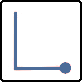
\includegraphics[angle=0,width=0.1\linewidth,keepaspectratio='true']{figures/dr.png}}] BD, comme un~L~: Affiche la fenêtre de dialogue de sélection du point de virage, similaire à l'élément du menu ``\textbf{L}iste de points de virage''.
\item[\raisebox{-1em}
{
\includegraphics[angle=0,width=0.1\linewidth,keepaspectratio='true']{figures/rd.png}}] DB, comme un~T~: Ouvre le gestionnaire de circuit (``\textbf{T}ask en anglais)
\item[\raisebox{-1em}
{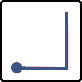
\includegraphics[angle=0,width=0.1\linewidth,keepaspectratio='true']{figures/dl.png}}] BG~: Affiche la liste des dégagements
\item[\raisebox{-1em}
{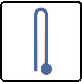
\includegraphics[angle=0,width=0.1\linewidth,keepaspectratio='true']{figures/ud.png}}] HB~: Active le zoom automatique
\end{itemize}
\vspace{2em}

\subsection*{Fenêtres de dialogue évoluées~:}
\begin{itemize}
\item[\raisebox{-1em}
{
\includegraphics[angle=0,width=0.1\linewidth,keepaspectratio='true']{figures/urd.png}}] HDB, comme un~A~: Affiche le fenêtre d'\textbf{A}nalyses.
\item[\raisebox{-1em}
{
\includegraphics[angle=0,width=0.1\linewidth,keepaspectratio='true']{figures/ldrdl.png}}] GBDBG, comme un ~S~: Affiche le fenêtre d'états (``\textbf{S}tatus'' en anglais).
\end{itemize}

